\documentclass[a4paper,10pt]{article}
\usepackage[utf8]{inputenc}
\usepackage[pdftex]{graphicx}
\usepackage{caption}
\usepackage{subcaption}

%opening
\title{Filtro Digital IIR utilizando aproximação Elíptica}
\author{Danilo Souza, Hugo Santos, Welton Araújo}

\begin{document}

\maketitle

\section{Introdução}
Existe uma necessidade muito grande em processamento de sinais em tratar sinais de entrada em uma determinada banda de frequência. Isto só é possível por meio de uma função de transferência com uma razão de polinômios para gerar filtros com resposta ao impulso de duração infinita(IIR).

Filtros IIR têm uma melhor aplicação prática por conta de precisar de menos multiplicações para realizar uma aproximação. Diferentemente de filtros com resposta ao impulso finitas(FIR), pois possuem mais dificuldade na atuação em processamento de sinais em tempo real.

O método de aproximação adotado neste trabalho, o elíptico, tem sua origem no domínio do tempo contínuo. Por conseguinte, é necessária uma transformação para o tempo discreto, através da transformação bilinear.

\section{Método da Transformação Bilinear}
Consiste no mapeamento da metade esquerda do plano \textit{s} dentro de uma circunferência unitária do plano \textit{z} através de uma normalização do espectro analógico da frequência de um intervalo \(-\infty < \Omega < \infty\) para \(-\pi < \omega < \pi\). Sua diferença do método da invariância ao impulso a resposta na frequência analógica é a indefinição do seu intervalo na frequência dentro da circunferência unitária.

Sua vantagem se deve ao fato de evitar o \textit{aliasing}, portanto mantém características da resposta ao módulo da função de transferência no tempo contínuo na transformação em função de transferência no tempo discreto. %Em resumo, o método da transformação bilinear ocorre da seguinte forma:

%\begin{itemize}
% \item Aplicar-se a pré-distorção nas frequências de passagem e rejeição, \(\omega_p\) e \(\omega_r\), respectivamente, específicas do filtro gerando novas frequências pré-distorcidas, \(\Omega_p\) e \(\Omega_r\).
% \item Gerar a função de transferência analógica \(H_a\)(s)
% \item FALTA O RESTO
% \end{itemize}

\begin{table}
\centering
\begin{tabular}{|l|l|}

\(A_p\) 	& 1 dB		\\
\(A_r\) 	& 40 dB		\\
\(\Omega_p\) 	& 1000 Hz	\\
\(\Omega_r\) 	& 1290 Hz	\\
\(\Omega_s\) 	& 3000 Hz	\\

\end{tabular}
\caption{Propriedades do filtro I}
\label{tab:tabfiltro1}
\end{table}

\section{Filtro I}
Trata-se de um filtro passa-baixa. Suas especificações estão inseridas na Tabela \ref{tab:tabfiltro1}. Onde \(A_p\) e \(A_r\) são a atenuação máxima e mínima nas frequências de passagem e rejeição, respectivamente. E \(\Omega_p\), \(\Omega_r\) e \(\Omega_s\) são as frequências de máxima de passagem, mínima de rejeição e de amostragem, respectivamente. 
 

A equação de diferença gerada por esse filtro é: 
\[y[n+5] - 4,546y[n+4] + 8,419y[n+3] - 7,928y[n+2] \]
\[- 3,793y[n+1] - 0,7372y[n] = 0,00733x[n+5] - 0,01843x[n+4]\]
\[ + 0,01149x[n+3] + 0,01149x[n+2] - 0,01843x[n+1] + 0,00733x[n] \]

A expressão da transformada Z é:

\[0,00733z^5 - 0,01843z^4 + 0,01149z^3\]
\[+ 0,01149z^2 - 0,01843z^1 + 0,00733 \]
\hline
\[ z^5 - 4,546z^4 + 8,419z^3 - \]
\[7,928z^2 - 3,793z - 0,7372 \]
A expressão da transformada de Fourier é:
\[0,00733e^{jw5} - 0,01843e^{jw4}\]
\[ + 0,01149e^{jw3} + 0,01149e^{jw2} - 0,01843e^{jw} + 0,00733 \]
\hline
\[ e^{jw5} - 4,546e^{jw4} + 8,419e^{jw3} - 7,928e^{jw2}\] 
\[ - 3,793e^{jw} - 0,7372\]

\subsection{Implementação no MatLab}
Para achar a ordem do filtro foi feito primeiro a normalização das frequências de passagem
e de rejeição. Usando o método "ellipord" do matlab achou-se a ordem mínima n=5. Então para projetar
o filtro foi utilizado o método "ellip" do matlab colocando respectivamente: a ordem do filtro,
a atenuação de passagem, a atenuação de rejeição, e a frequência de corte(que é igual a frequência
de passagem) foi adicionado o paramêtro 's' para se criar um filtro analógico.

Com os parmêtros do numerador e denominador do filtro analógico foi usado o método "bilinear" para
fazer o mapeamento do tempo contínuo para o discreto. Para achar a equação da função de transfêrencia
foi usado o metodo 'tf' e foi passado os coeficientes do numerador e denominador do filtro discreto.
Para pegar os gráficos de módulo e fase e resposta ao impulso foi usada a função "fvtool".


Os gráficos das respostas em frequência em magnitude, magnitude normalizada e fase estão nas Figuras \ref{fig:magnitude1} e \ref{fig:fase1}.

\begin{table}[ht]
\centering
\begin{tabular}{|l|l|}

\(A_p\) 	& 0,5 dB	\\
\(A_r\) 	& 60 dB		\\
\(\Omega_p1\) 	& 40 rad/s	\\
\(\Omega_r1\) 	& 50 rad/s	\\
\(\Omega_p2\) 	& 70 rad/s	\\
\(\Omega_r2\) 	& 80 rad/s	\\
\(\Omega_s\) 	& 240 rad/s	\\

\end{tabular}
\caption{Propriedades do filtro II}
\label{tab:tabfiltro2}
\end{table}


\section{Filtro II}
Trata-se de um filtro rejeita-faixa. Suas especificações estão inseridas na Tabela \ref{tab:tabfiltro2}. Onde \(A_{p1}\) e \(A_{r1}\) são a atenuação máxima e mínima nas frequências de passagem e rejeição, respectivamente. \(\Omega_{p1}\) e \(\Omega_{r1}\) são as frequências  máxima de passagem e mínima de rejeição, respectivamente, da faixa inicial. \(\Omega_{p2}\), \(\Omega_{r2}\) são as frequências mínima de passagem, máxima de rejeição, respectivamente, da faixa final.
A frequ\^encia de amostragem \'e representada por \(\Omega_s\)

A equação de diferença gerada por esse filtro é: 
\[        y[n+10]	- 0,2185y[n+9] 		+ 1,726y[n+8] 		- 0,3473y[n+7]\]
\[+  1,929y[n+6] 	- 0,2756y[n+5] 		+ 0,9223y[n+4] 		- 0,1009y[n+3]\]
\[+ 0,3202y[n+2] 	- 0,004673y[n+1] 	+ 0,03496y[n] =		      \]

\[  0,1988x[n+10] 	- 0,06244x[n+9] 	+ 0,9305y[n+8] 		- 0,2366x[n+7]\]
\[+  1,802x[n+6] 	- 0,3488x[n+5] 		+ 1,802x[n+4] 		- 0,2366x[n+3]\]
\[+ 0,9305x[n+2] 	- 0,06244x[n+1] 	+ 0,1988x[n]			      \] 

A expressão da transformada Z é:
\[  0,1988z^{10} 	- 0,06244z^9 		+ 0,9305z^8 		- 0,2366z^7\]
\[+  1,802z^6 		- 0,3488z^5 		+ 1,802z^4 		- 0,2366z^3\]
\[+ 0,9305z^2 		- 0,06244z^1 		+ 0,1988			   \]
\hline
\[        z^{10} 		- 0,2185z^9 		+ 1,726z^8 		- 0,3473z^7\]
\[+  1,929z^6 		- 0,2756z^5 		+ 0,9223z^4 		- 0,1009z^3\]
\[+ 0,3202z^2		- 0,004673z 		- 0,03496			   \]

A expressão da transformada de Fourier é:
\[  0,1988e^{jw10} 	- 0,06244e^{jw9} 	+ 0,9305e^{jw8} 	- 0,2366e^{jw7}\]
\[+  1,802e^{jw6} 	- 0,3488e^{jw5} 	+ 1,802e^{jw4} 		- 0,2366e^{jw3}\]
\[+ 0,9305e^{jw2} 	- 0,06244e^{jw} 	+ 0,1988  			       \]
\hline
\[        e^{jw10} 	- 0,2185e^{jw9} 	+ 1,726e^{jw8} 		- 0,3473e^{jw7}\]
\[+  1,929e^{jw6} 	- 0,2756e^{jw5} 	+ 0,9223e^{jw4} 	- 0,1009e^{jw3}\]
\[+ 0,3202e^{jw2} 	- 0,004673e^{jw} 	- 0,03496			       \]

\subsection{Implementação no MatLab}
No caso desse filtro que é um rejeita-faixa, foi calculado as frequencias normalizadas de passagem e de rejeição para que
fosse possível encontrar a ordem do filtro usando a função "ellipord", após isso foi criado um filtro passa-baixa equivalente com o método "ellip"

Após isso foi usado o método "lp2bs" para fazer a criação do filtro rejeita-faixa equivalente ainda no tempo contínuo. Tendo
a função de transferência contínua foi usado novamente o método "bilinear" para que fosse criado o mapeamento no tempo discreto.
foi usado novamente a função "tf" para achar a função de transferência e o "fvtool" para achar os gráficos equivalentes.

Os gráficos das respostas em frequência em magnitude e fase estão nas Figuras \ref{fig:magnitude2} e \ref{fig:fase2}.

\begin{figure}[ht]
 \centering
 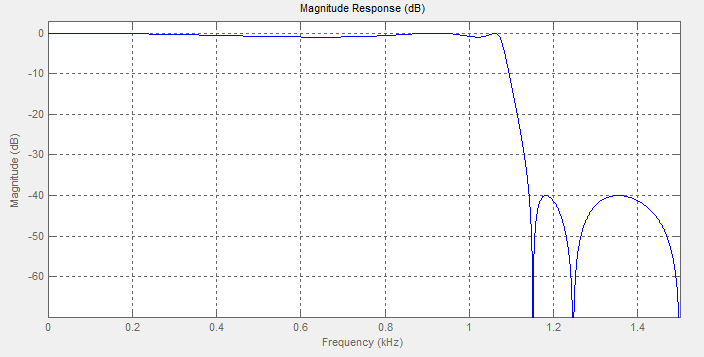
\includegraphics[width=12cm]{pictures/Filtro1/Magnitude.png}
 \caption{Resposta em frequência em magnitude do filtro I}
 \label{fig:magnitude1}
\end{figure}

\begin{figure}[ht]
 \centering
 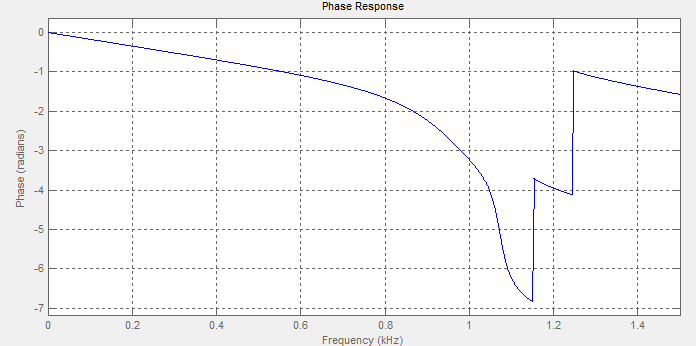
\includegraphics[width=12cm]{pictures/Filtro1/Fase.png}
 \caption{Resposta em frequência em fase do filtro I}
 \label{fig:fase1}
\end{figure}

O gráfico da resposta ao impulso e o diagrama de polos e zeros estão nas figuras \ref{fig:resimp1} e \ref{fig:diapolozero1}, respectivamente.

\begin{figure}[ht]
 \centering
 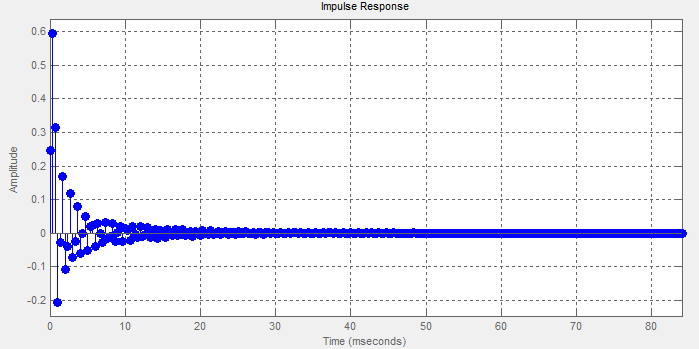
\includegraphics[width=12cm]{pictures/Filtro1/RespImpulso.png}
 \caption{Resposta ao impulso do filtro I}
 \label{fig:resimp1}
\end{figure}

\begin{figure}[ht]
 \centering
 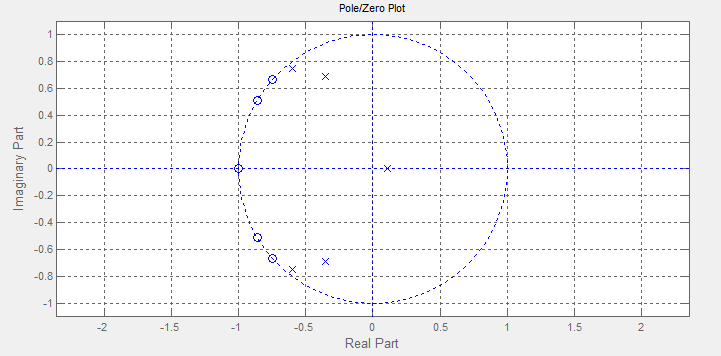
\includegraphics[width=10cm]{pictures/Filtro1/Polos&Zeros.png}
 \caption{Diagrama de polos e zeros do filtro I}
 \label{fig:diapolozero1}
\end{figure}

\begin{figure}[ht]
 \centering
 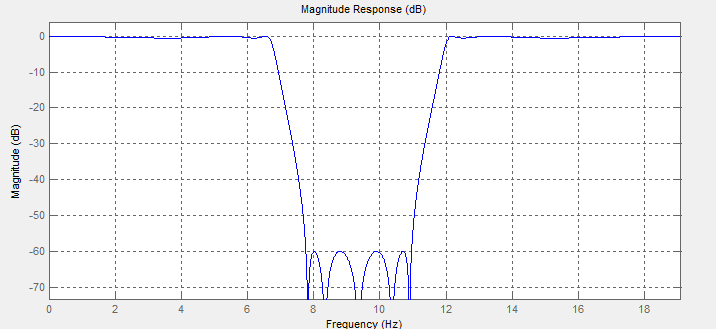
\includegraphics[width=12cm]{pictures/Filtro2/Magnitude.png}
 \caption{Resposta em frequência em magnitude do filtro II}
 \label{fig:magnitude2}
\end{figure}

\begin{figure}[ht]
 \centering
 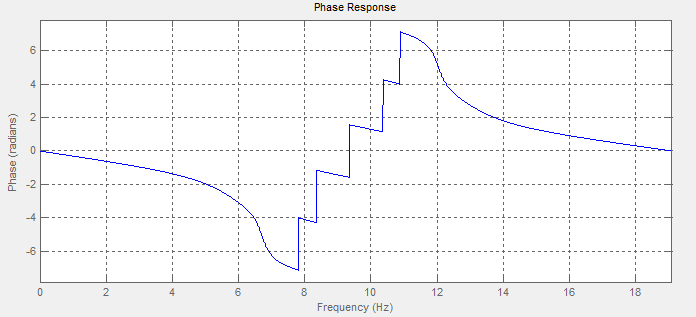
\includegraphics[width=12cm]{pictures/Filtro2/Fase.png}
 \caption{Resposta em frequência em fase do filtro II}
 \label{fig:fase2}
\end{figure}

O gráfico da resposta ao impulso e o diagrama de polos e zeros estão nas figuras \ref{fig:resimp2} e \ref{fig:diapolozero2}, respectivamente.

\begin{figure}[ht]
 \centering
 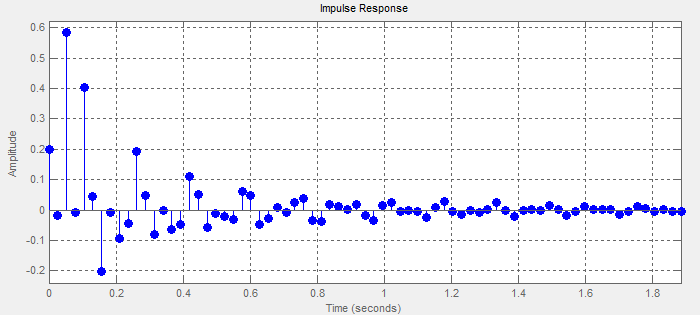
\includegraphics[width=12cm]{pictures/Filtro2/RespImpulso.png}
 \caption{Resposta ao impulso do filtro II}
 \label{fig:resimp2}
\end{figure}

\begin{figure}[ht]
 \centering
 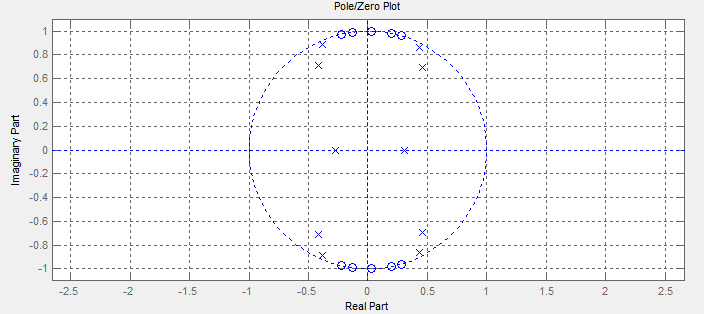
\includegraphics[width=12cm]{pictures/Filtro2/Polos&Zeros.png}
 \caption{Diagrama de polos e zeros do filtro II}
 \label{fig:diapolozero2}
\end{figure}



\end{document}
